\appendix{Представление графического материала}

Графический материал, выполненный на отдельных листах,
изображен на рисунках А.1--А.\arabic{числоПлакатов}.
\setcounter{числоПлакатов}{0}

\renewcommand{\thefigure}{А.\arabic{figure}} % шаблон номера для плакатов
\begin{landscape}
	
	\begin{плакат}
		
\includegraphics[width=0.82\linewidth]{титульник.eps}
		\заголовок{Сведения о ВКРБ}
		\label{pl1:image}      
	\end{плакат}
	
\begin{плакат}
	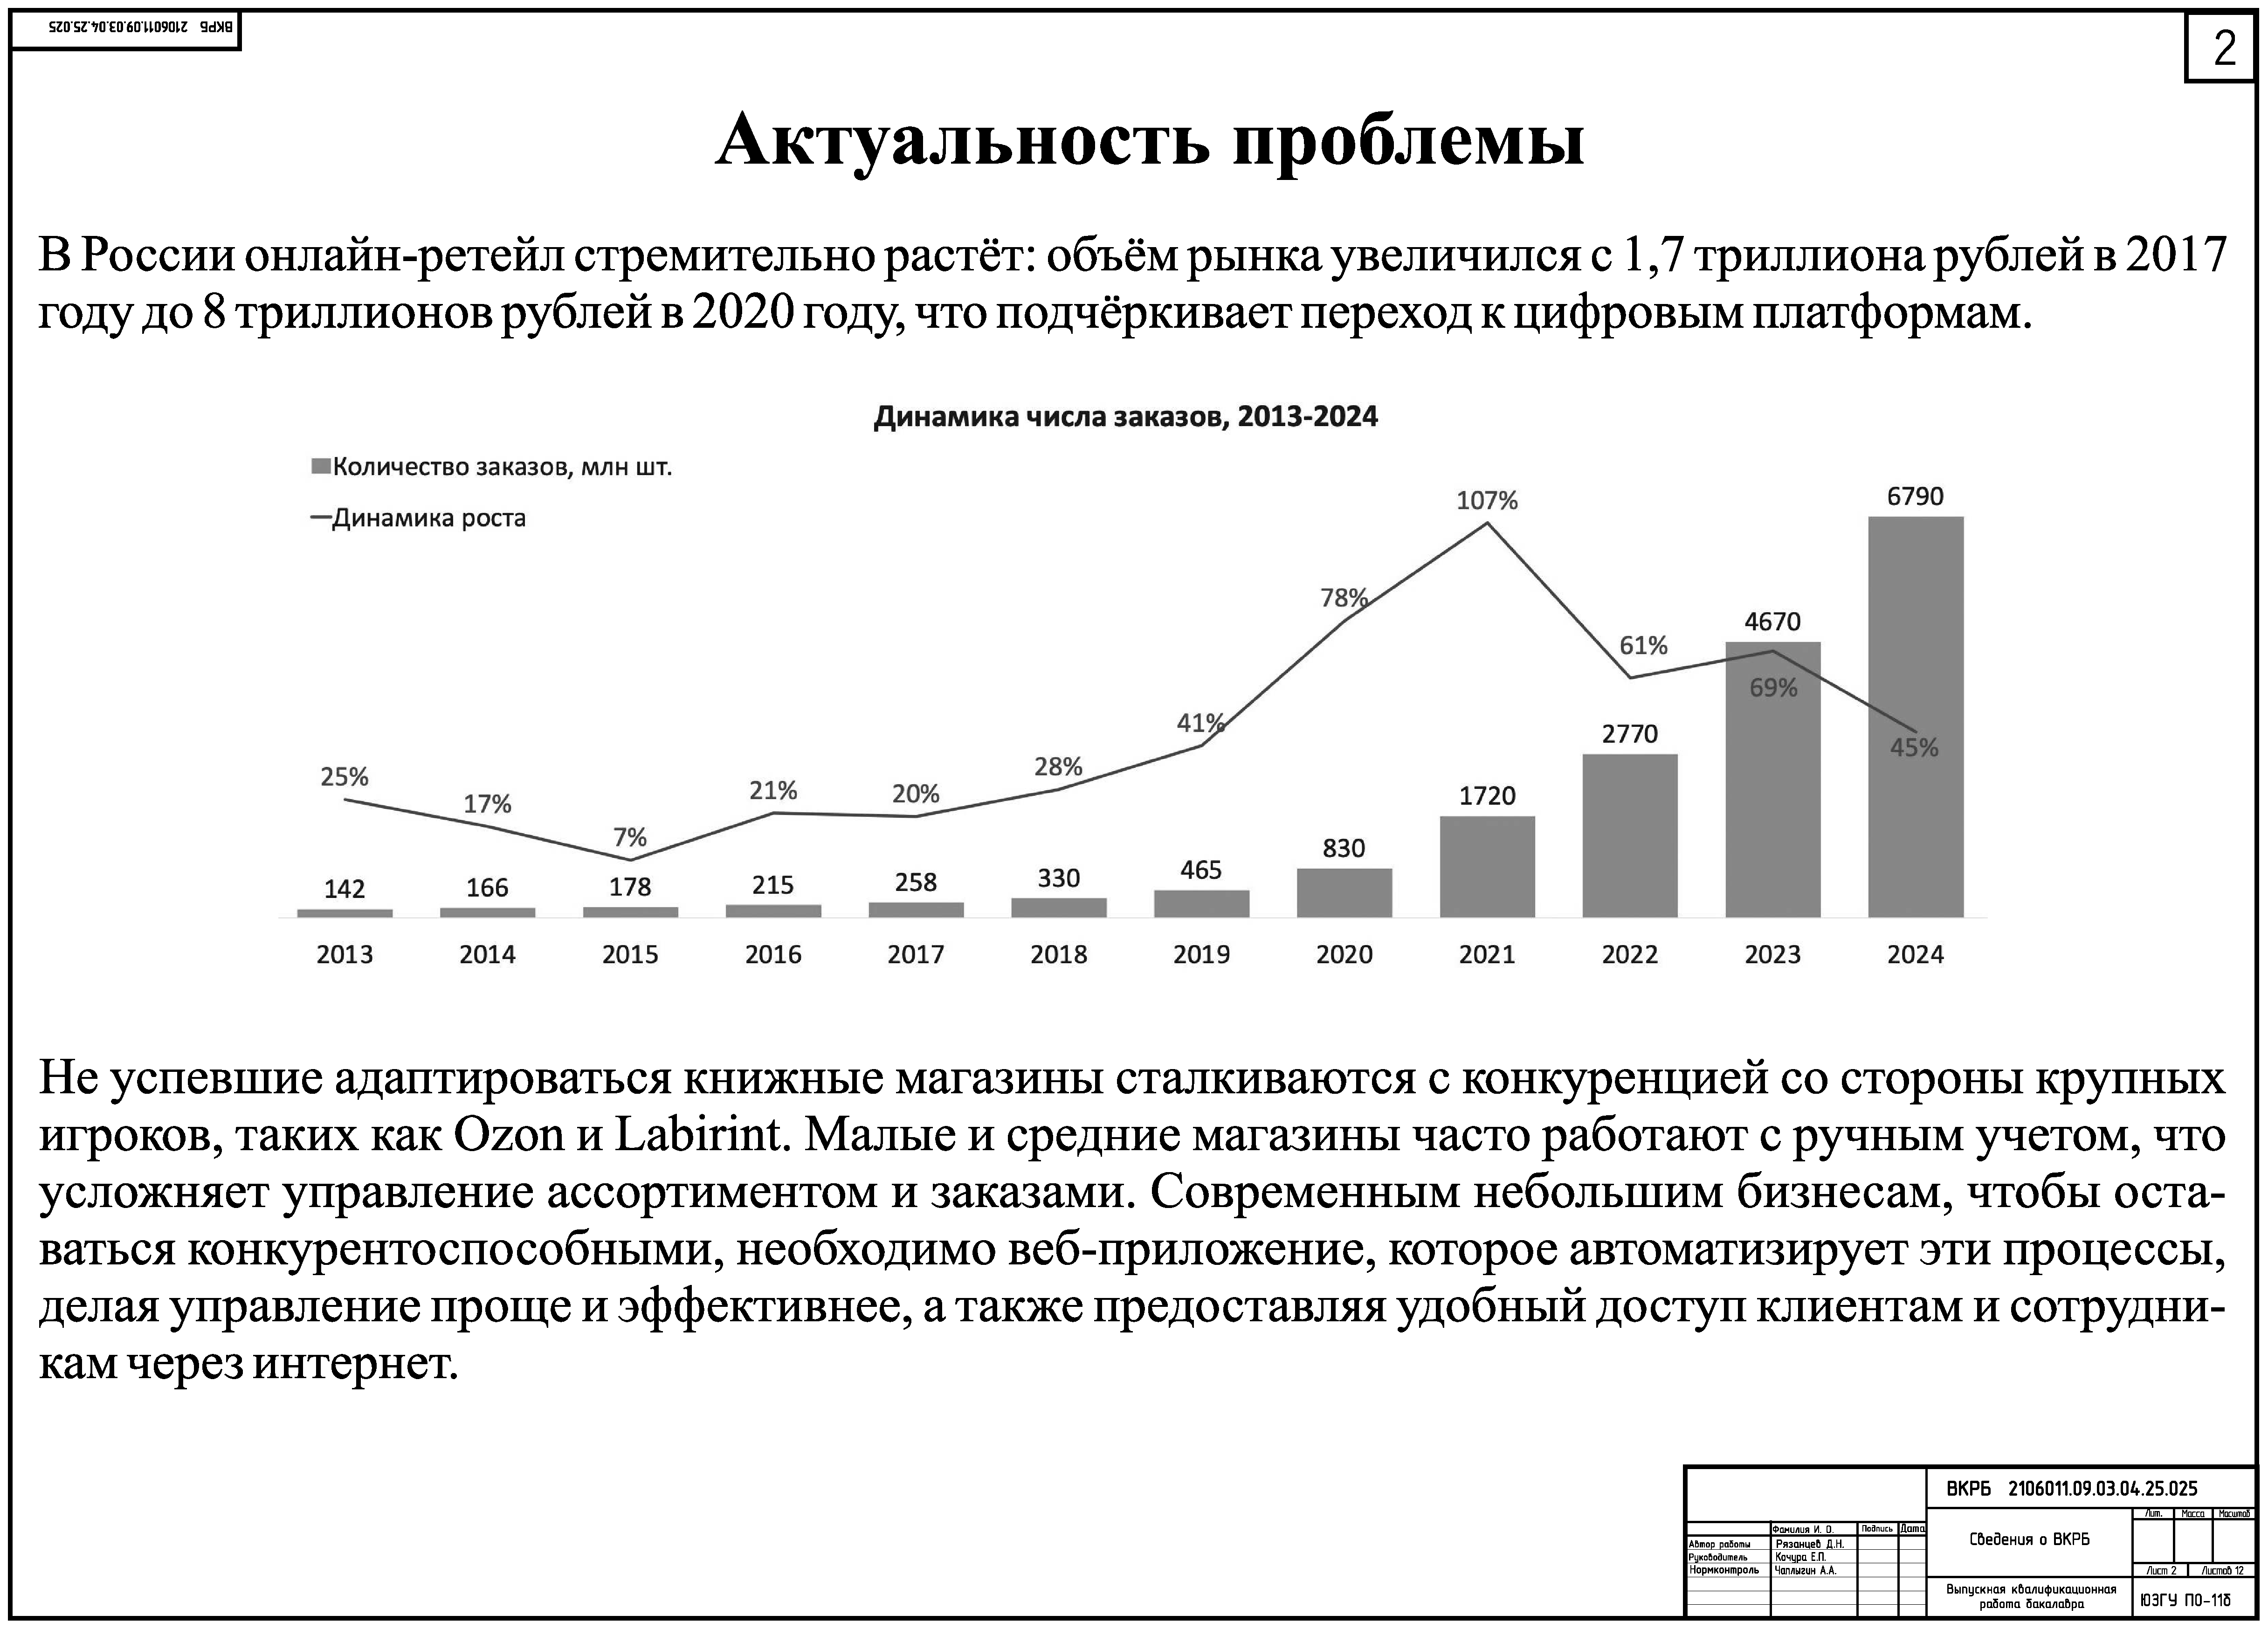
\includegraphics[width=0.82\linewidth]{2.eps}
	\заголовок{Актуальность проблемы}
	\label{pl2:image}      
\end{плакат}

\begin{плакат}
	
\includegraphics[width=0.82\linewidth]{3.eps}
	\заголовок{Цель и задачи работы}
	\label{pl3:image}      
\end{плакат}

\begin{плакат}
	
\includegraphics[width=0.82\linewidth]{4.eps}
	\заголовок{Концептуальная модель данных}
	\label{pl4:image}      
\end{плакат}

\begin{плакат}
	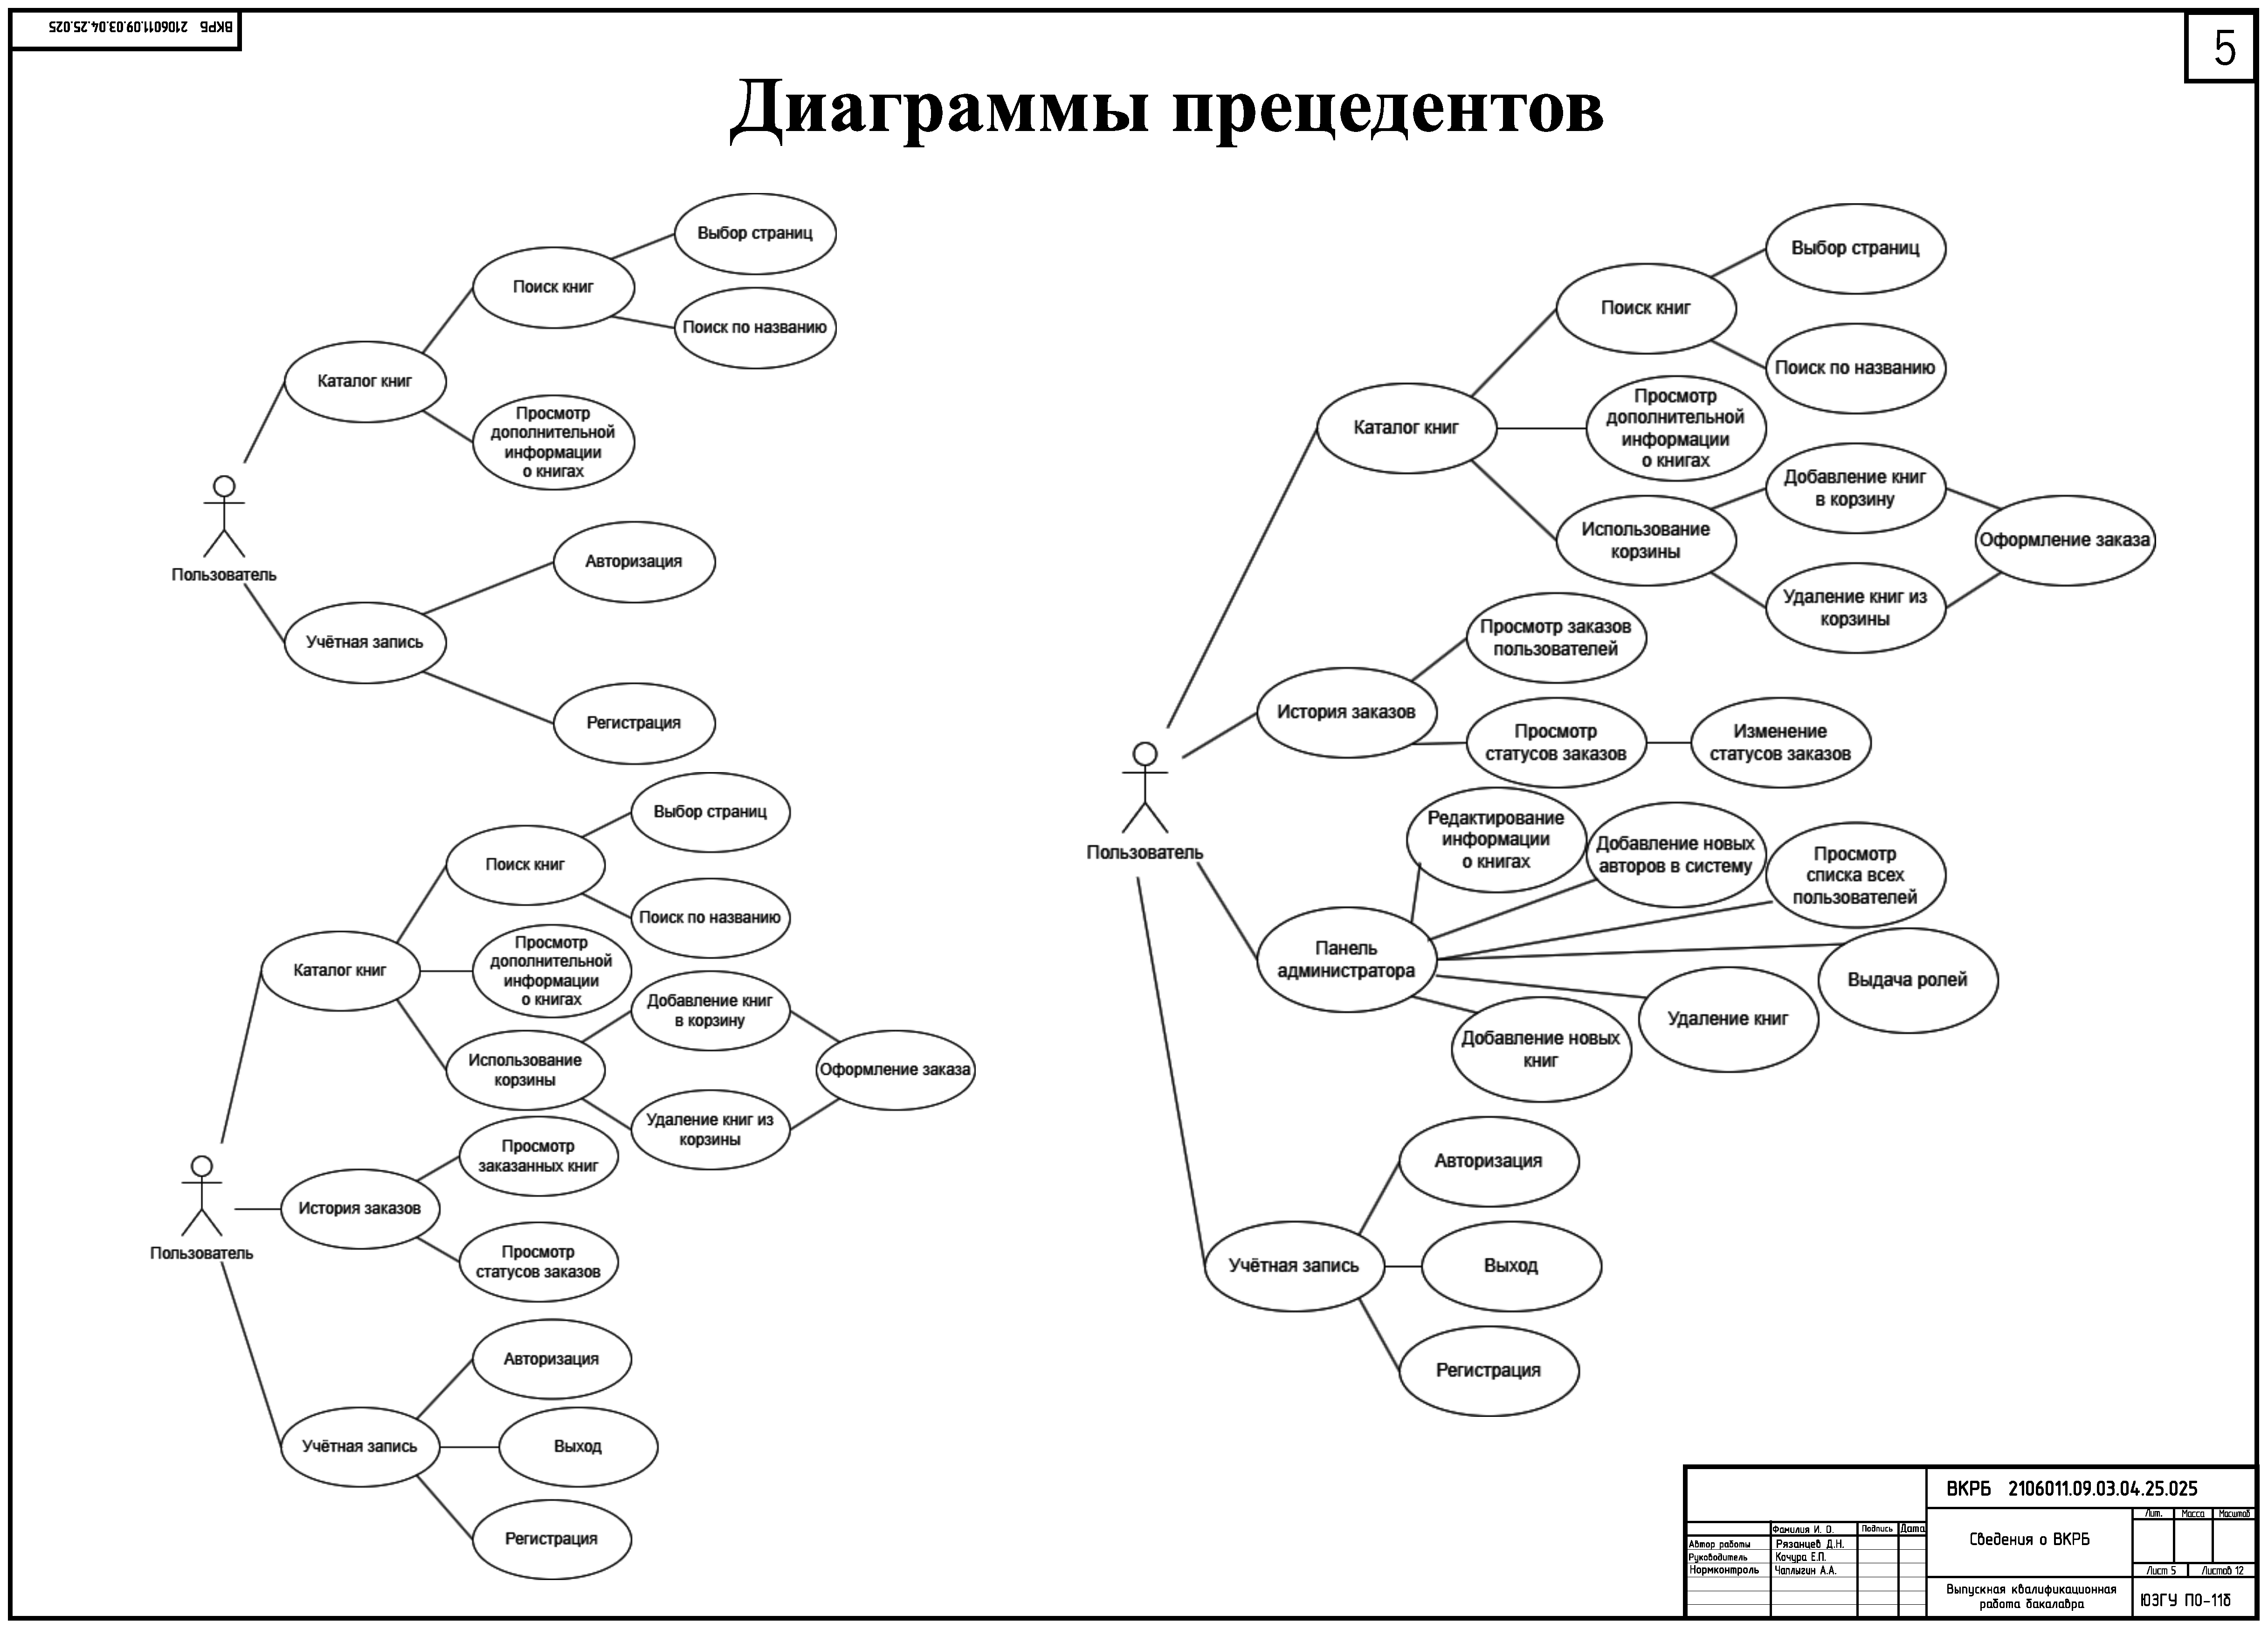
\includegraphics[width=0.82\linewidth]{5.eps}
	\заголовок{Диаграммы прецедентов}
	\label{pl5:image}      
\end{плакат}

\begin{плакат}
	
\includegraphics[width=0.82\linewidth]{6.eps}
	\заголовок{Архитектура интеллектуальной системы}
	\label{pl6:image}      
\end{плакат}

\begin{плакат}
	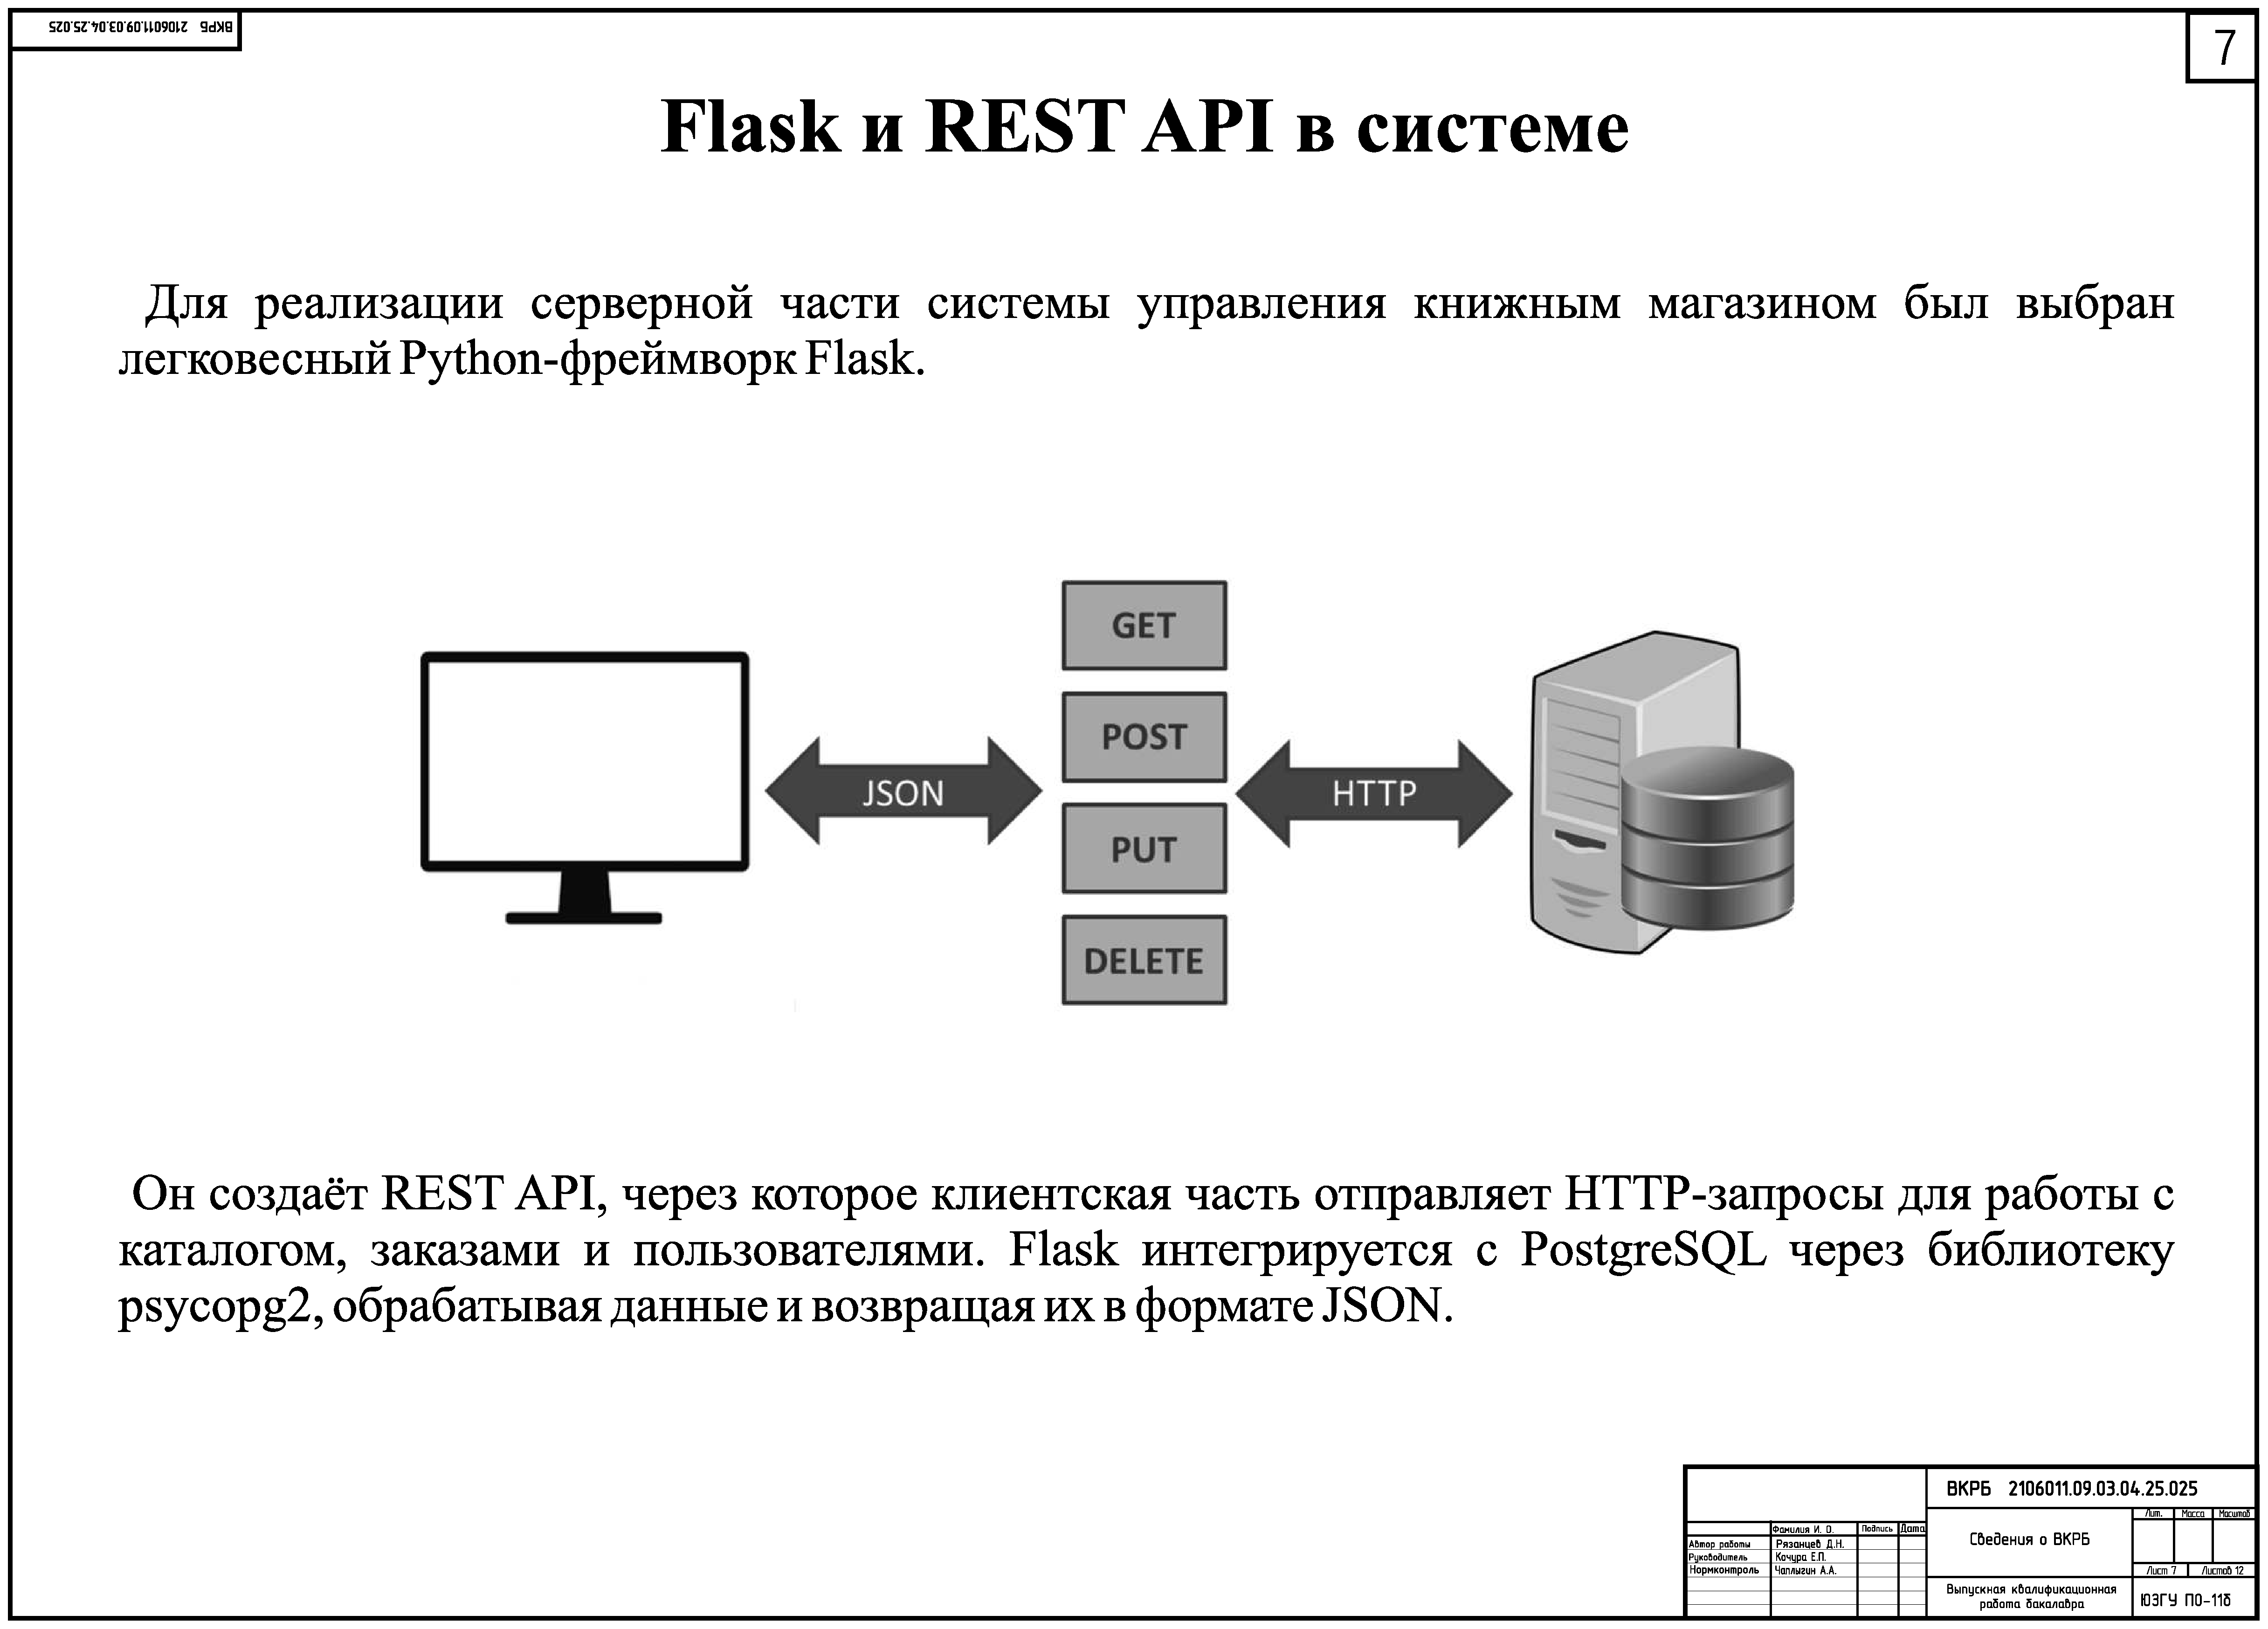
\includegraphics[width=0.82\linewidth]{7.eps}
	\заголовок{Flask и REST API в системе}
	\label{pl7:image}      
\end{плакат}

\begin{плакат}
	
\includegraphics[width=0.82\linewidth]{8.eps}
	\заголовок{Интерфейс веб-приложения}
	\label{pl8:image}      
\end{плакат}

\begin{плакат}
	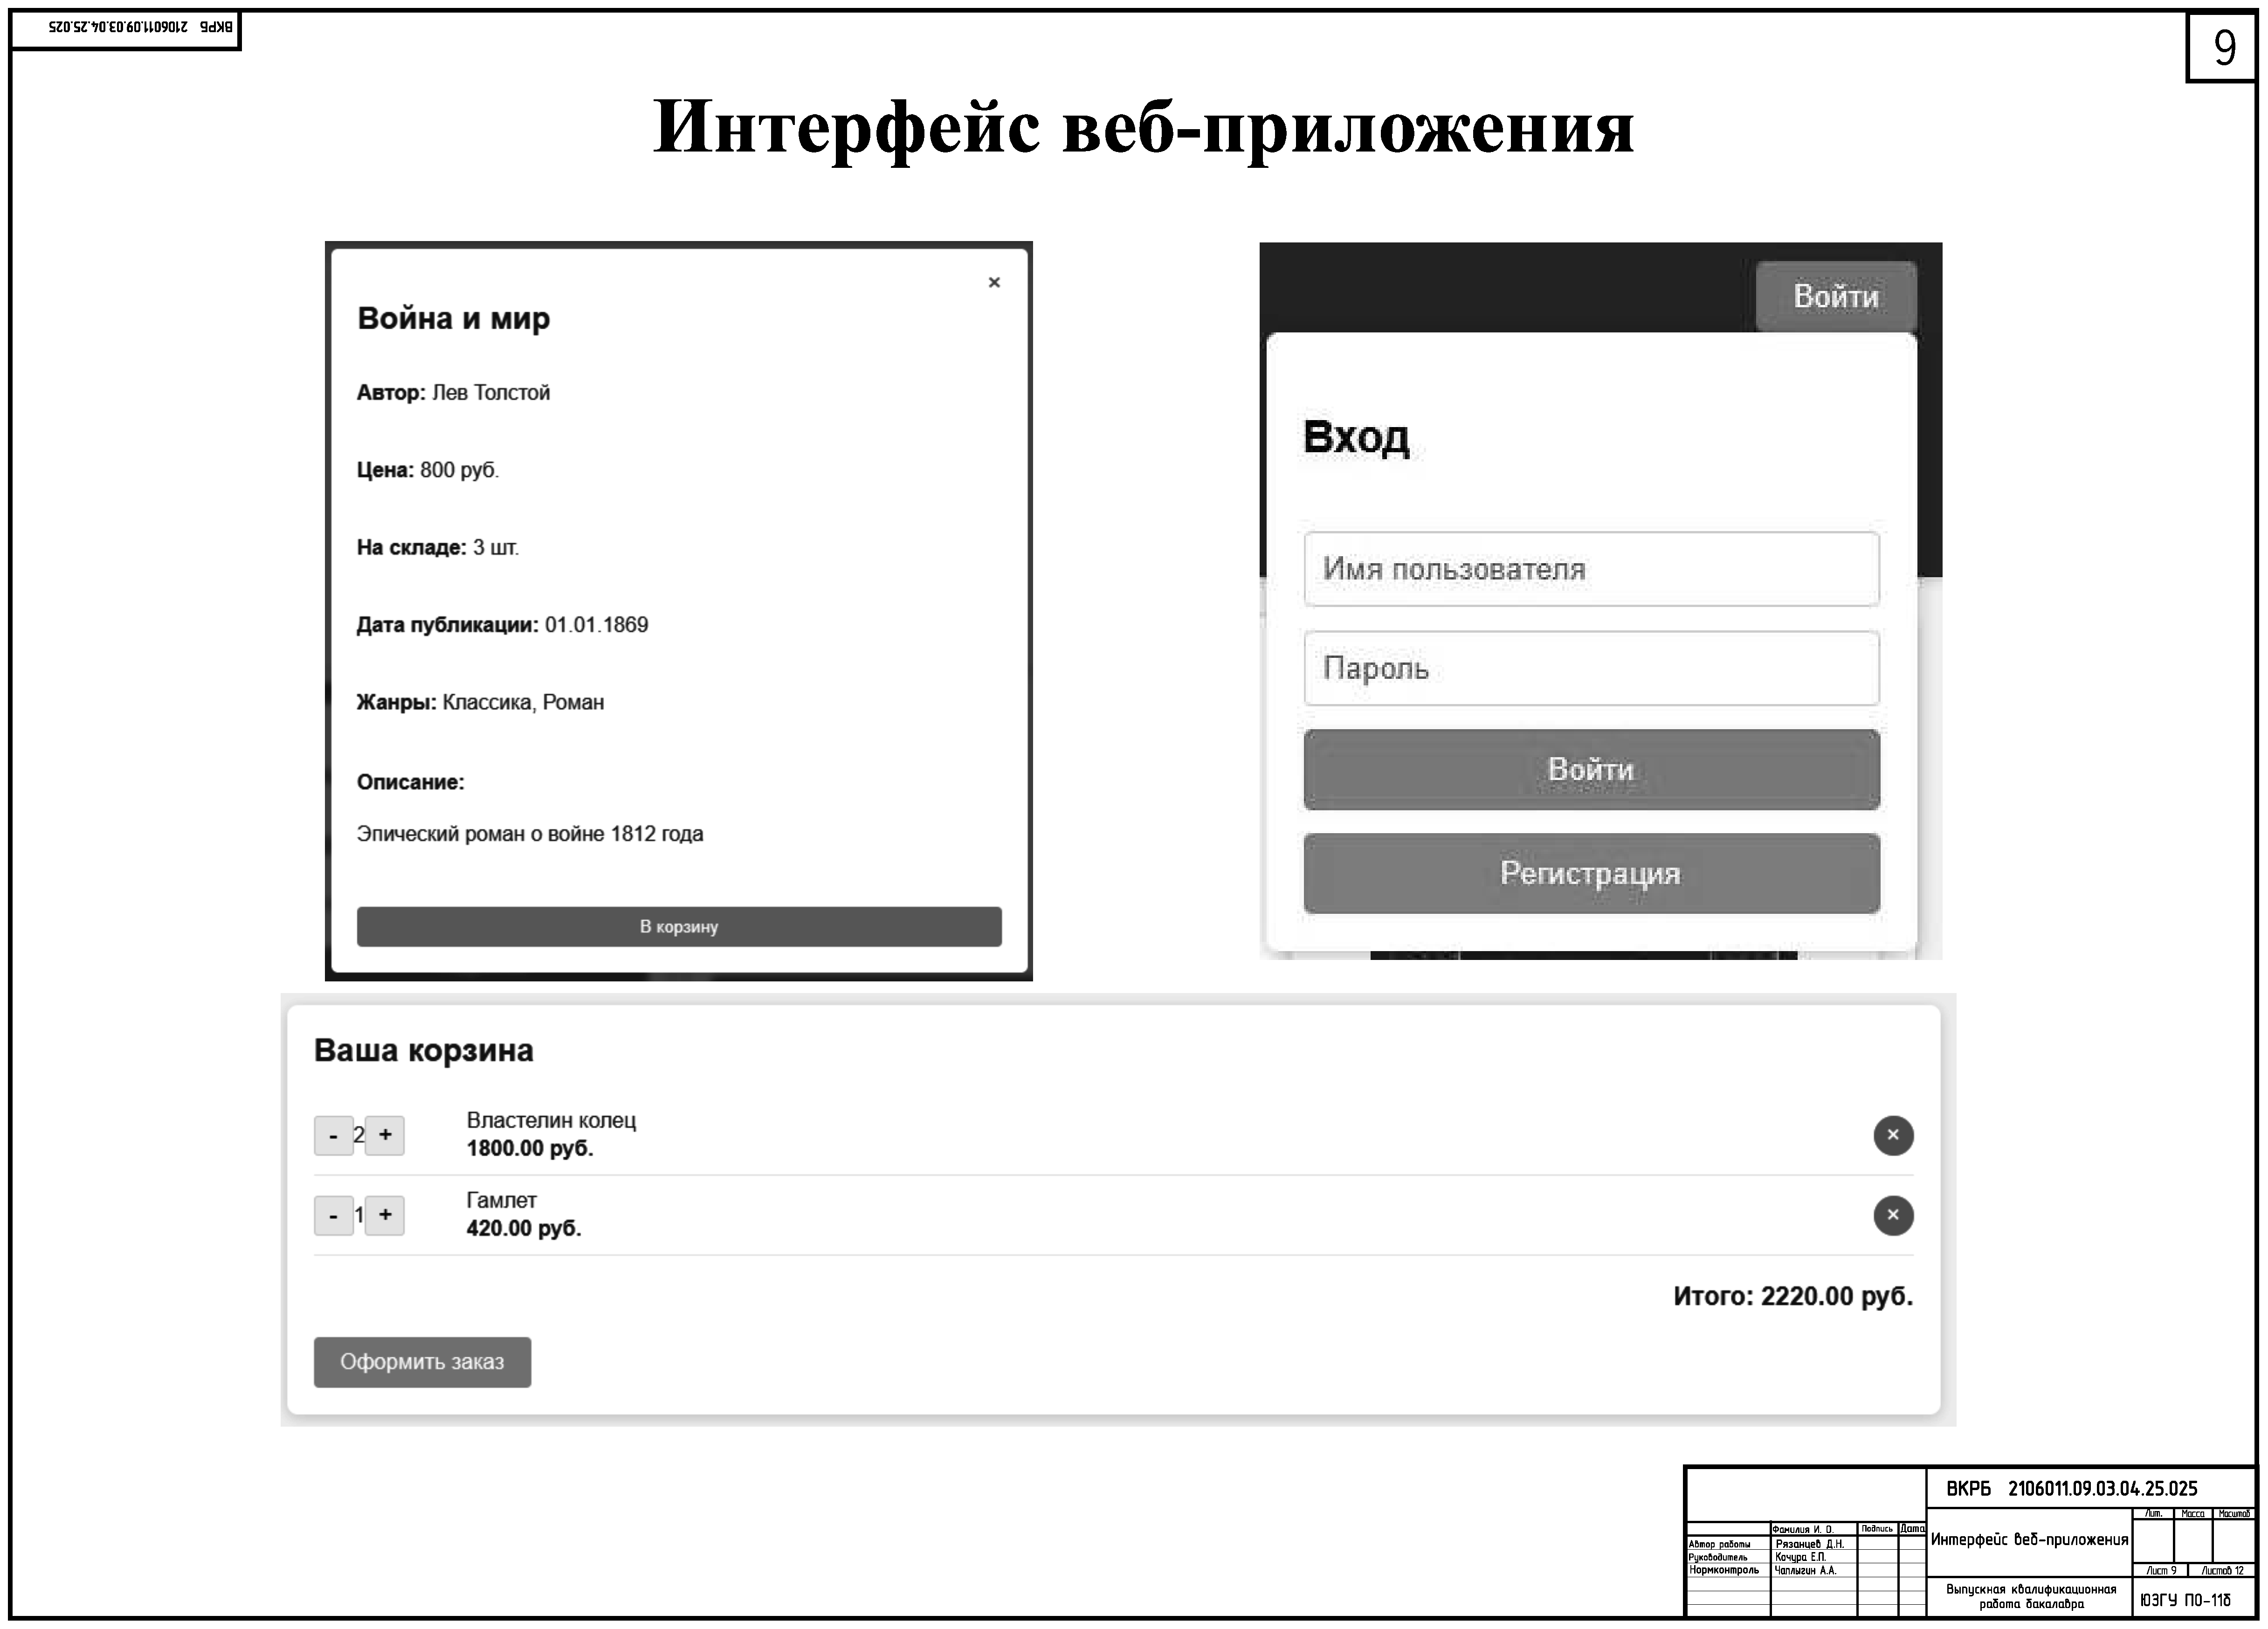
\includegraphics[width=0.82\linewidth]{9.eps}
	\заголовок{Интерфейс веб-приложения}
	\label{pl9:image}      
\end{плакат}

\begin{плакат}
	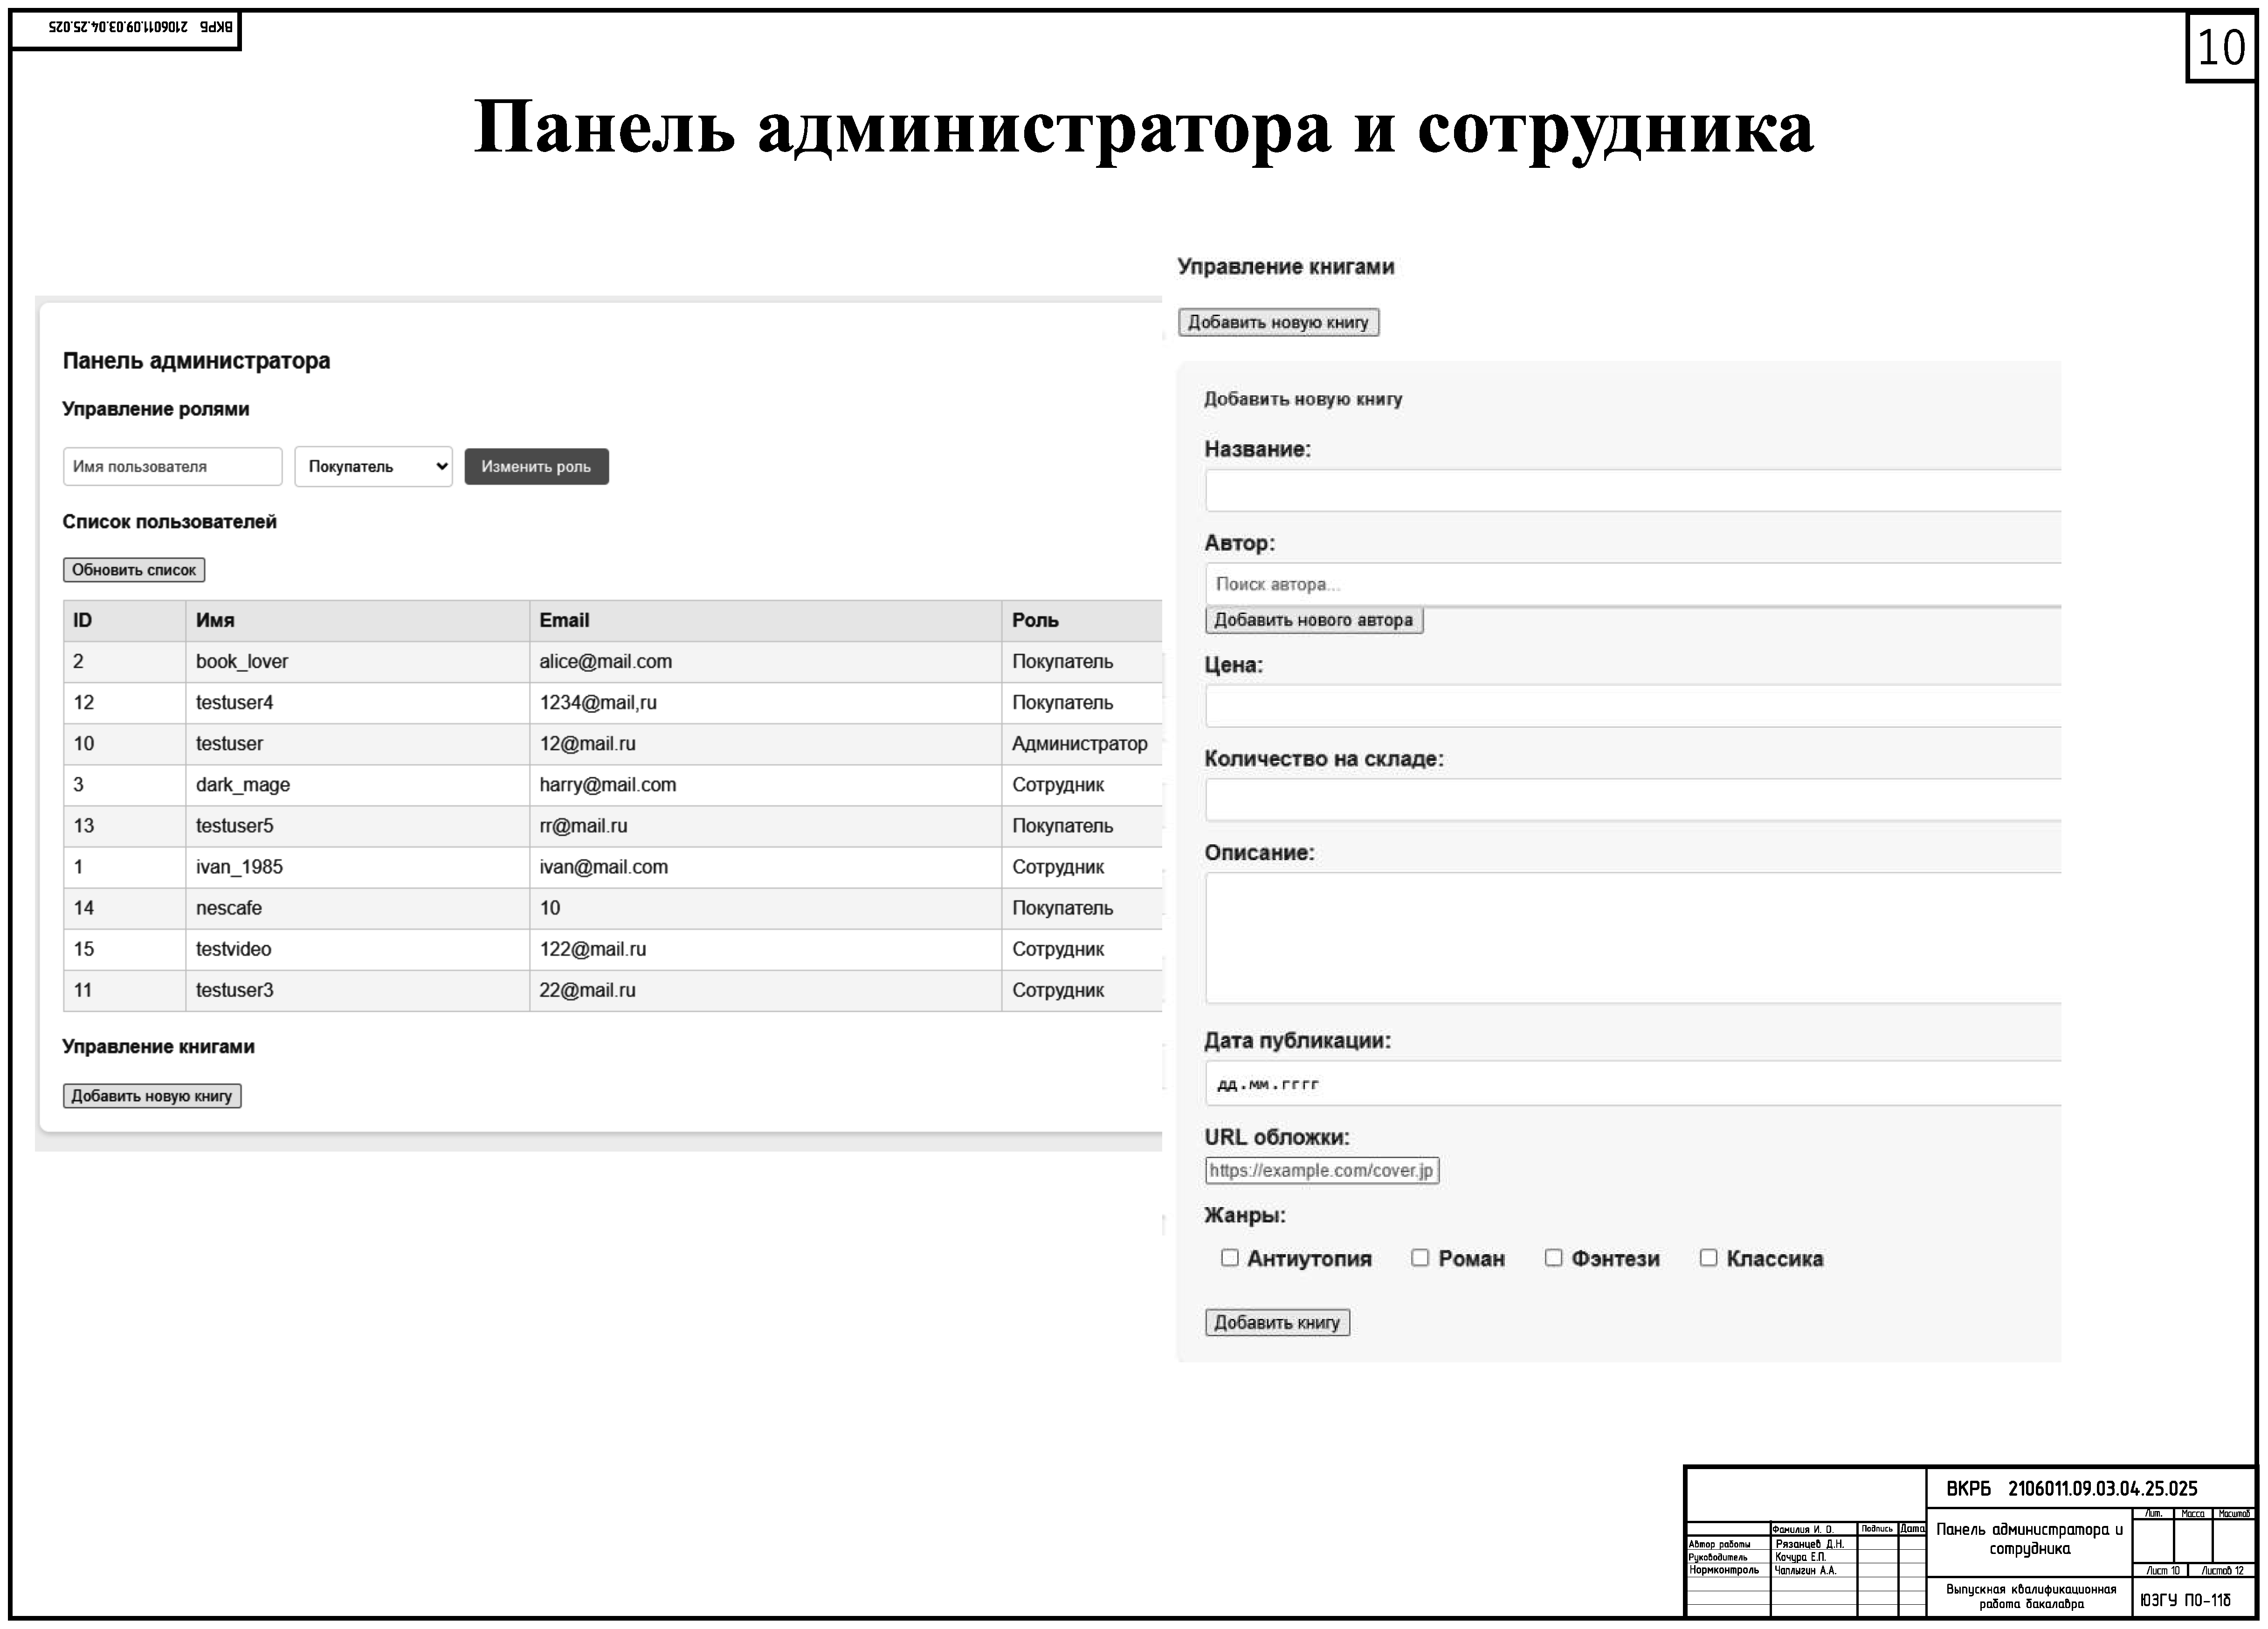
\includegraphics[width=0.82\linewidth]{10.eps}
	\заголовок{Панель администратора и сотрудника}
	\label{pl10:image}      
\end{плакат}

\begin{плакат}
	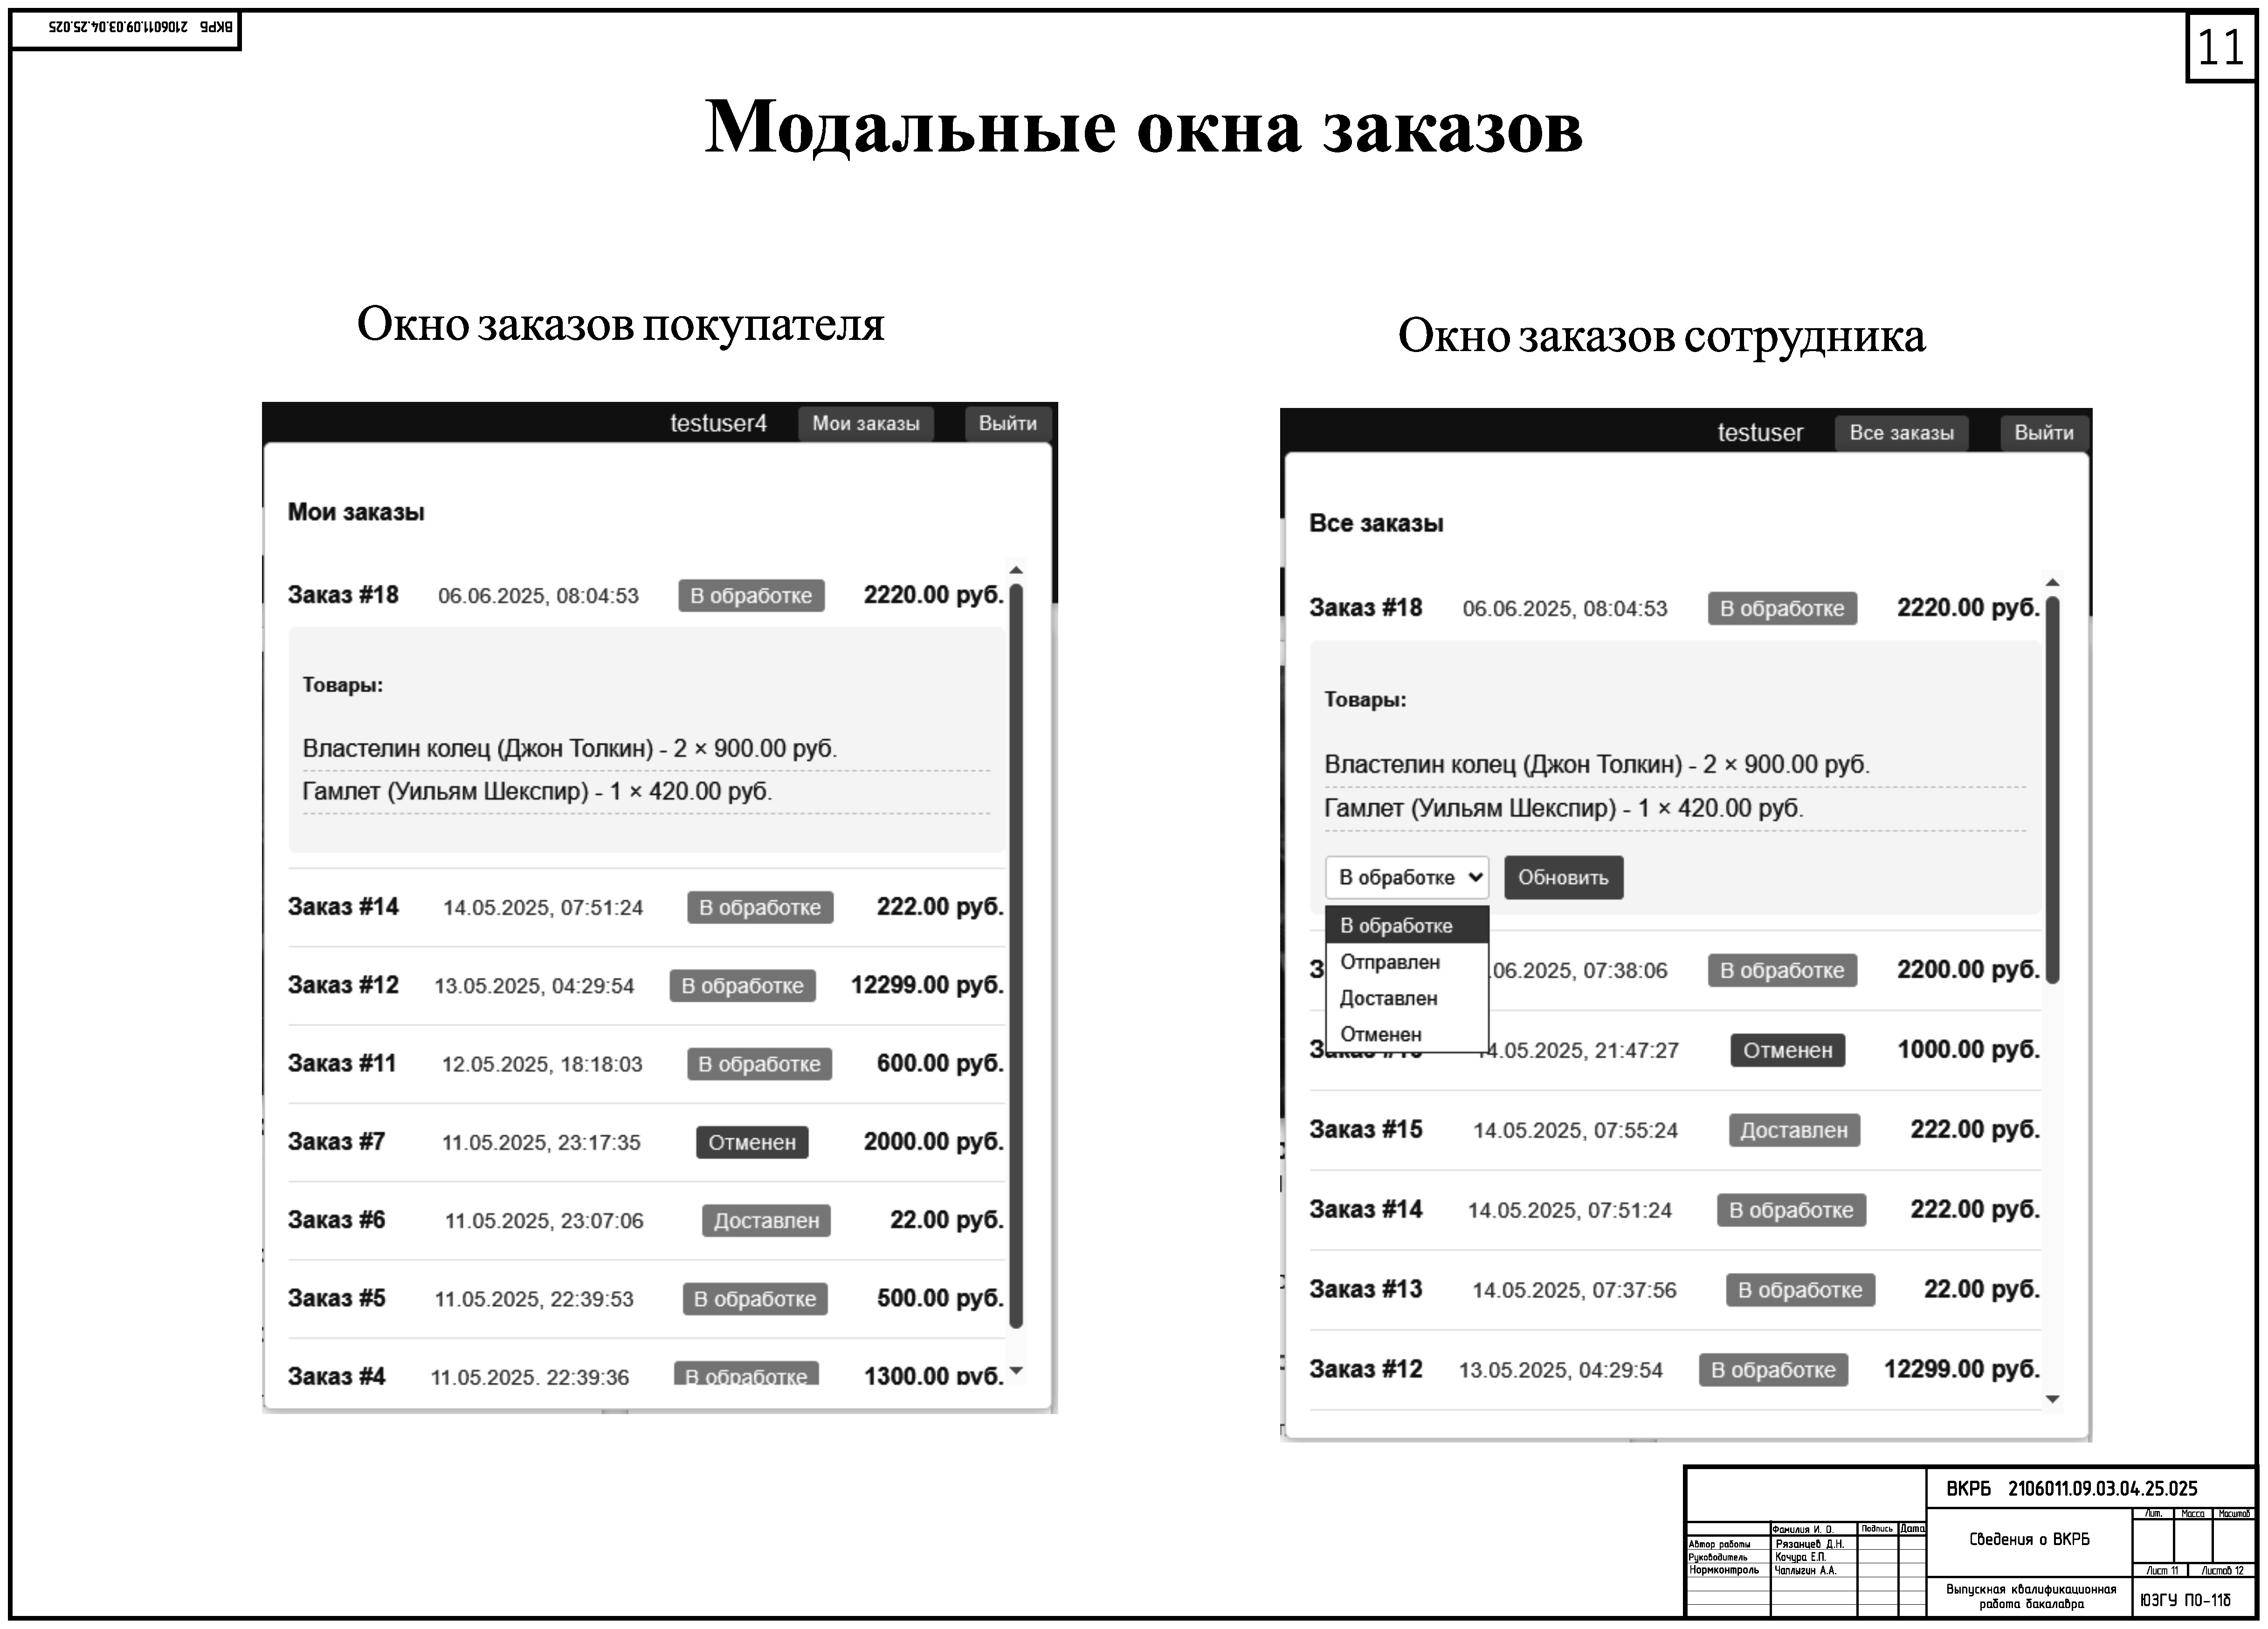
\includegraphics[width=0.82\linewidth]{11.eps}
	\заголовок{Модальные окна заказов}
	\label{pl11:image}      
\end{плакат}

\begin{плакат}
	
\includegraphics[width=0.82\linewidth]{12.eps}
	\заголовок{Заключение}
	\label{pl12:image}      
\end{плакат}












\end{landscape}